El programa fue planteado como una maquina de estados, existiendo nueve estados diferentes. A su vez, cada estado es tratado como una FSM más pequeña.

\begin{figure}[H]
\centering
	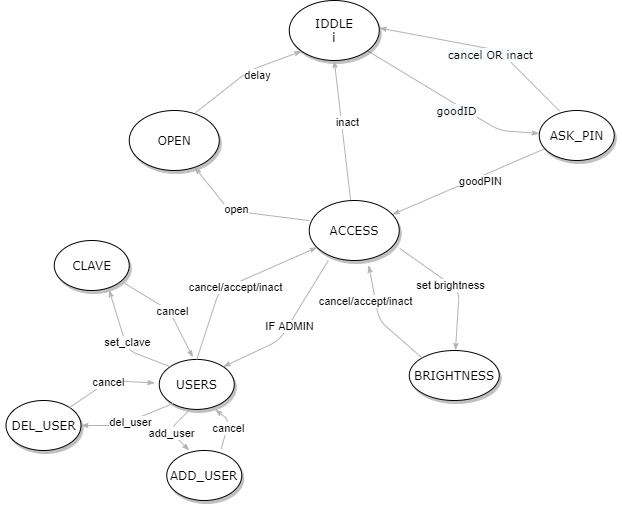
\includegraphics[width=0.6\textwidth]{ImagenesEjercicio2/fsm.png}
	\caption{FSM del programa.}
	\label{fig:fsm}
\end{figure}

El estado \textbf{IDDLE} es el estado principal por defecto, en el cual se debe ingresar un ID empleando tanto las dos alternativas posibles (mediante encoder o mediante la tarjeta). Al realizar la validación de dicha ID, se pasa al estado \textbf{ASK PIN}.

\begin{figure}[H]
\centering
	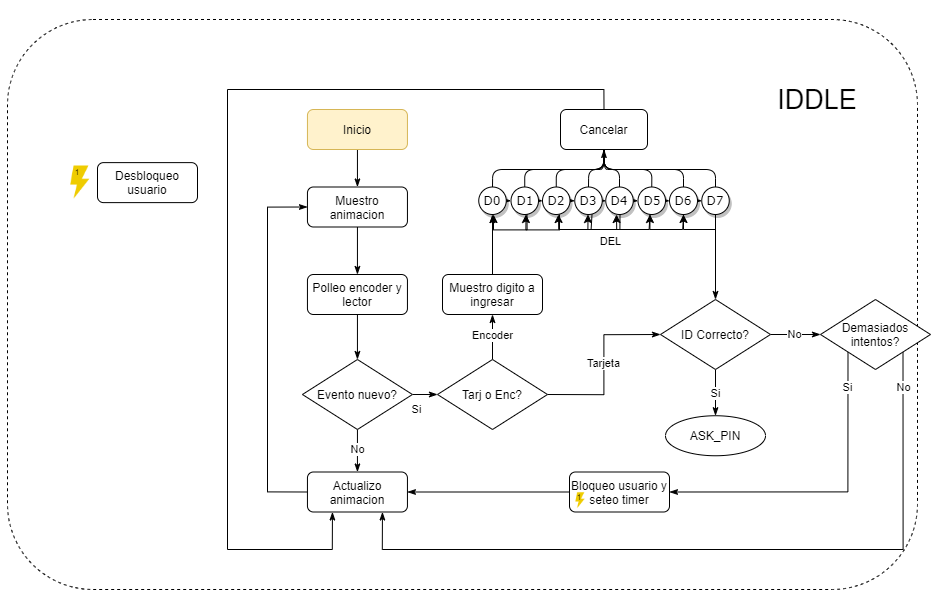
\includegraphics[width=0.6\textwidth]{ImagenesEjercicio2/iddle.png}
	\caption{FSM del estado \textbf{IDDLE}.}
	\label{fig:iddle}
\end{figure}

El estado \textbf{ASK PIN} se obtiene el pin de acceso del usuario, que las ser validado se continua al estado de \textbf{ACCES}.

\begin{figure}[H]
\centering
	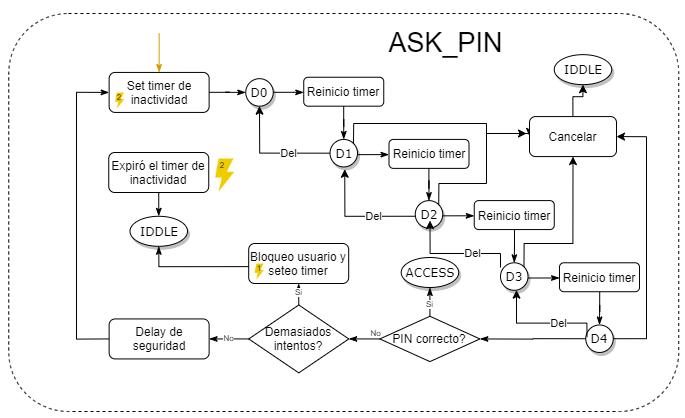
\includegraphics[width=0.6\textwidth]{ImagenesEjercicio2/askpin.png}
	\caption{FSM del estado \textbf{ASK PIN}.}
	\label{fig:askpin}
\end{figure}

En \textbf{ACCESS} puede retornarse al estado \textbf{IDDLE} (luego de cierto período de inactividad), al acceso de del edificio abriendo la puerta o a un panel de configuración del sistema.

\begin{figure}[H]
\centering
	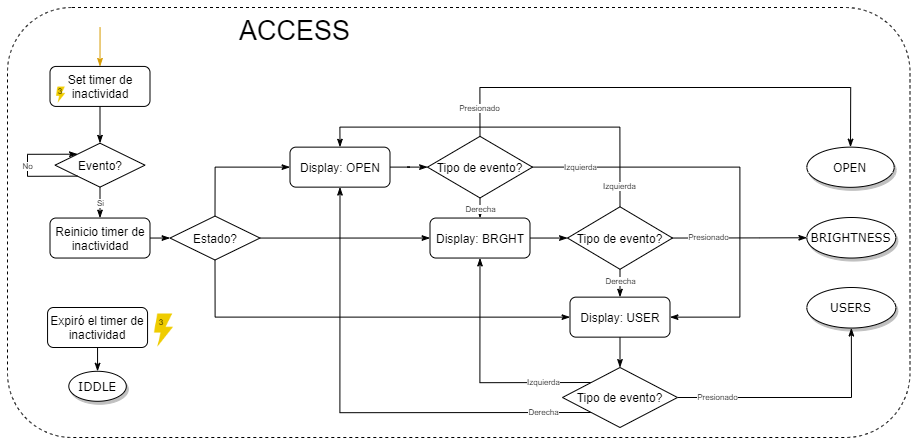
\includegraphics[width=0.6\textwidth]{ImagenesEjercicio2/access.png}
	\caption{FSM del estado \textbf{ACCESS}.}
	\label{fig:access}
\end{figure}

Dicho panel de configuración se encuentra conformado por dos estados distintos, siendo estos el estado \textbf{BRIGHTNESS} y \textbf{USERS}. El primero permite cambiar el brillo del display empleado, mientras que el segundo otorga ciertas configuraciones diferenciadas.

\begin{figure}[H]
\centering
	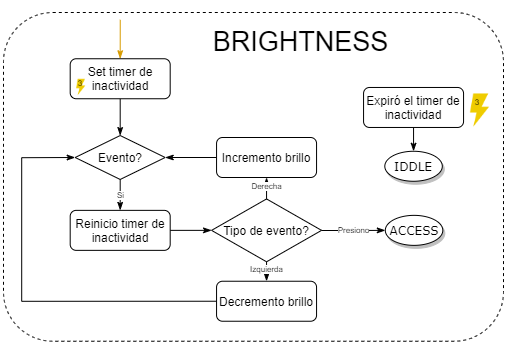
\includegraphics[width=0.6\textwidth]{ImagenesEjercicio2/bright.png}
	\caption{FSM del estado \textbf{BRIGHTNESS}.}
	\label{fig:bright}
\end{figure}

Cabe destacar que cualquier usuario puede acceder tanto a la configuración del brillo como de usuarios, pero dentro de este último estado existen ciertas limitaciones.

\begin{figure}[H]
\centering
	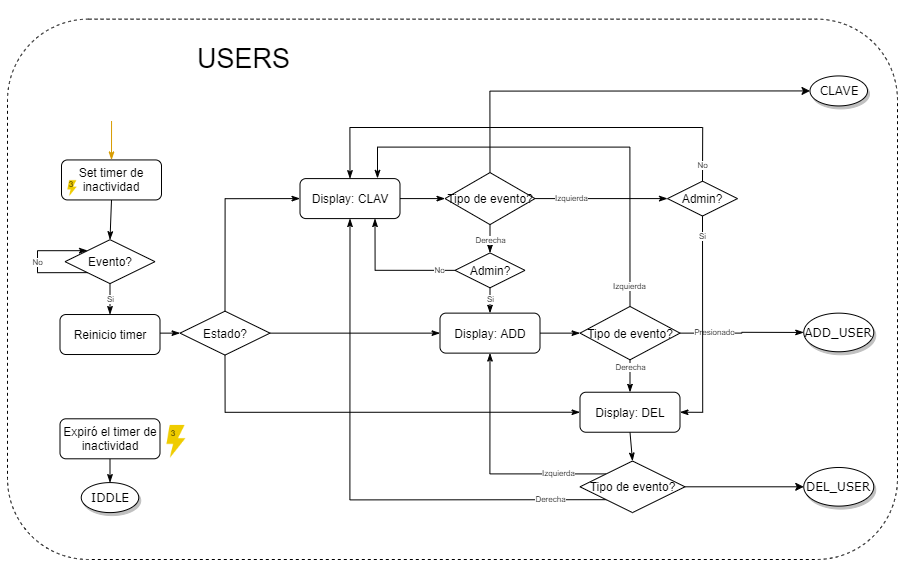
\includegraphics[width=0.6\textwidth]{ImagenesEjercicio2/users.png}
	\caption{FSM del estado \textbf{USERS}.}
	\label{fig:users}
\end{figure}

Cualquier persona puede acceder al estado \textbf{CLAVE}, donde puede cambiar su propio pin de seguridad. Pero solo los que cuentan con el rango de administrador son los que tienen acceso a los dos estados restantes. 

\begin{figure}[H]
\centering
	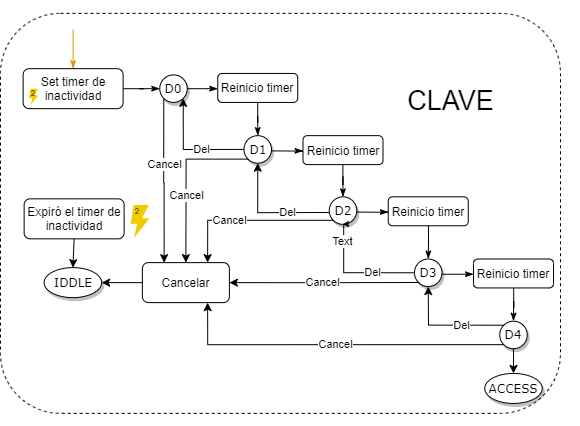
\includegraphics[width=0.6\textwidth]{ImagenesEjercicio2/clave.png}
	\caption{FSM del estado \textbf{CLAVE}.}
	\label{fig:clave}
\end{figure}

Los estados exclusivos de \textbf{ADD USER} y \textbf{DEL USER} permiten que cualquier administrador agregue a un nuevo usuario o elimine a uno existente respectivamente.

\begin{figure}[H]
\centering
	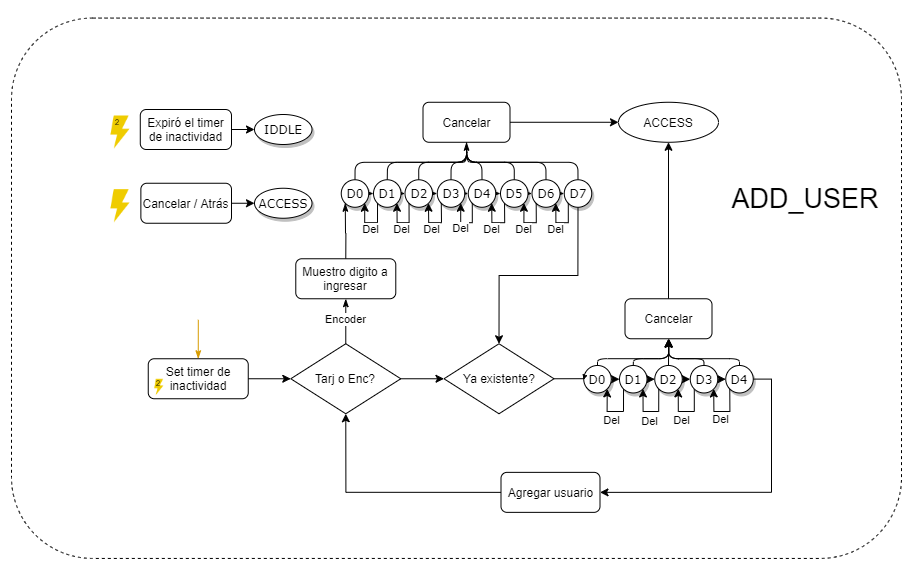
\includegraphics[width=0.6\textwidth]{ImagenesEjercicio2/adduser.png}
	\caption{FSM del estado \textbf{ADD USER}.}
	\label{fig:adduser}
\end{figure}

\begin{figure}[H]
\centering
	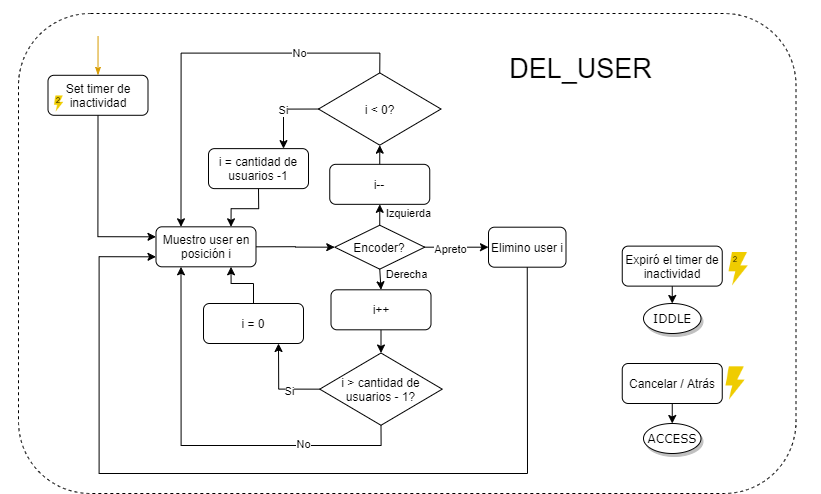
\includegraphics[width=0.6\textwidth]{ImagenesEjercicio2/deluser.png}
	\caption{FSM del estado \textbf{DEL USER}.}
	\label{fig:deluser}
\end{figure}